INTRO: 
	- Different ways of realizing them
	- CZ gate


\chapter{Calibrating and Characterizing Controlled Arbitrary Phase Gates}
This chapter details the purpose, calibration and characterization of \glspl{carb}. We start by explaining how they can benefit \glspl{vqa} and how they can be seen as extension of standard \glspl{cz}. Next, we demonstrate the implementation of a \glspl{carb} on a physical device and detail its calibration procedure. By exploiting the 3-level readout discussed in Chapter \ref{ch:qutrit_readout}, we then characterize conditional-/dynamic- phase errors and leakage, and compare these values to the ones obtained with a \gls{cz} implemented on the same qubits.  In addition, we perform quantum process tomography for several angles and evaluate the gate fidelity for each angle.  We conclude that the gate performance is sufficient for its envisioned usage in \glspl{vqa} and implement such experiment in Chapter \ref{ch:qaoa}.


TODO: read iswap, johannes Thesis ch cphase gate.

\section{Motivation}
- intro two qubit gate: 
	- Role in algorithm; clifford group (?)  --> just subset is enough for computation, implies decomposition of more complex gates. 
	- In NISQ, this can be a problem due to decoherence
- in specific cases, might be useful to have something else than two standard clifford group to make it gate/time efficient. 
- in this work, investigate one case applied to Variation Quantum Algorithms. Other recent example iswap.

\section{Theoretical description}
For a pair of qubit $A$ and $B$, bringing the \oo state close to the \tz state the interaction Hamiltonian yields the following propagator \cite[p.~87]{Heinsoo2018}: 
\begin{equation}
    \begin{aligned}
U(t)=& e^{-i t J(|20\rangle\langle 11 |+|  11 \rangle \langle 20|)} \\
=& \mathrm{I}+\left[\cos \left(J t\right)-1\right](|11\rangle\langle 11|+| 20\rangle\langle 20|)-\\
& i \sin \left(J t\right)(|20\rangle\langle 11|+| 11\rangle\langle 20|)
\end{aligned}
\end{equation}
 where $J$ denotes the coupling strength between the \oo and the \tz state. Near resonance, the population is fully swapped back to the \oo state for
 \begin{equation}
     t_{\textrm{gate}} = \frac{2\pi} { \sqrt { \Delta ^ { 2 } + 4 J ^ { 2 } } }
 \end{equation} 
 and the corresponding geometric phase on the \oo state acquired by the closed loop state evolution is 
 \begin{equation}
     \phi_{ c } = \pi + \frac{\Delta \cdot t_{\textrm{gate}}}{2} = \pi \cdot \left( 1 + \frac { \Delta } { \sqrt { \Delta ^ { 2 } + 4 J ^ { 2 } } } \right)
 \end{equation}
 with $\Delta = \omega_{\ket{20}} - \omega_{\ket{11}}$ the frequency detuning between the \tz and \oo state. Hence, arbitrary phases can be reached by varying $\Delta$.
 
 Assuming qubit $B$ is fluxed with a pulse of amplitude $a$, $\Delta$ is related to the amplitude through the qubit frequency $\omega _ { | 01 \rangle }(a)$:
 \begin{equation}
\begin{aligned} 
\Delta(a) & = \omega _ { | 20 \rangle } - \omega _ { | 11 | \rangle } \\ 
& = 2 \omega _ { | 10 \rangle } - \alpha _ { A } - \left( \omega _ { | 10 \rangle } + \omega _ { | 01 \rangle }(a) \right) \\ 
& = \omega _ { | 10 \rangle } - \alpha _ { A } - \omega _ { | 01 \rangle }(a) 
\end{aligned}
\end{equation}
Recalling that
\begin{equation}
    \omega_{\ket{01}} \simeq \sqrt{8E_J E_c} - E_c
\end{equation}
and 
\begin{equation}
    E_J = E _ { J , \max } \sqrt { \cos ^ { 2 } \left( \frac { \partial \Phi } { \partial V } a \right) + d ^ { 2 } \sin ^ { 2 } \left( \frac { \partial \Phi} { \partial V } a \right) }
\end{equation}
where $\alpha_A$ denotes the anharmonicity of qubit $A$. $\gamma$

TODO: read Dicarlo, 
- restate CZ hamiltonian, show that by tuning amplitude and interaction time, we can change the phase to arbitrary value. 
- Chevron pattern --> Need high pop recovery.

Interaction hamiltonian and unitary
Fig: ?
\section{Calibration} 

In this section we report the different steps required to calibrate a \gls{carb} using unipolar, flat-top Gaussian flux pulses on qubit 2 and 3 of the device presented in Appendix \ref{app:setup}.

- Pulse parametrization: flat top gaussian. good for chevron but potentially accumulates changes on bias-T (not Net Zero). 
 Check up to which depth we can go. + need to introduce IIR and FIR filters. + buffers.

The implementation of a \gls{carb} relies on the same principle as the one of a \gls{cz}, namely the collection of geometric phase on the \oo state\footnote{For the implemented gate, $\ket{ij}$ is a short notation for qubit 2 and qubit 3 in states $i$ and $j$ respectively.} due to the interaction of the \oo level and the non-computational \tz level REF STRAUCH DICARLO. The geometric phase acquired by the \oo state during the gate depends on the frequency detuning between the \oo and \tz levels REF HEINSOO. At the qubit parking positions, the detuning is large such that the acquired phase is small (ideally zero). During the gate, we apply a flux pulse to one of the qubits. The pulse shifts the transition frequencies such that the \oo and \tz levels are closer to one another. By varying the amplitude of the flux pulse, we can change the frequency detuning of the interacting levels, and thus the collected phase. The interaction between the two levels also mediates a periodic population exchange between the \oo and \tz states, in addition to the geometric phase of interest. To ensure maximal \oo-state population recovery after the gate, the length of the interaction with the \tz-state has to be a multiple of the population exchange period. The period also depends on the frequency detuning between the \oo and \tz state. 

Hence, before calibrating the pulse amplitudes resulting in the phases of interest, we find the pulse lengths resulting in maximal population recovery for various flux pulse amplitudes. To this extend, we prepare the \oo state and perform a two-dimensional sweep  of the flux pulse amplitude and length. For each amplitude and length, we measure the \e level population of qubit 2 after the flux pulse using 3-level readout. This results in a chevron pattern REF? shown in the background of Fig. \ref{fig:ch4_calibration_carb}a. Brighter areas correspond to high \e level population of qubit 2, indicating the population is fully swapped back from the \f level into the computational subspace. To find the (shortest) pulse lengths resulting in maximal population recovery, we fit for each pulse amplitude the \e level population oscillation to a cosine. We then retrieve the pulse length corresponding to the first maximum of the population oscillation. (SHOULD IT BE PART OF A FIGURE?)

- fit model with free parameters for dphidV. NOTE: where to put derivation of model ? Should I talk about the model (probably).

Thereafter, we measure the conditional phase acquired for different flux pulse amplitudes (see Fig. \ref{fig:ch4_calibration_carb}b). For each amplitude, the length of the pulse is set to the one obtained by the fit to the corresponding amplitude. For any amplitude in between calibration points, the pulse length is interpolated linearly. 
To visualize this effect, we overlay the measurement points of Fig. \ref{fig:ch4_calibration_carb}b on Fig. \ref{fig:ch4_calibration_carb}a at the corresponding amplitude and pulse length. The colored flux pulses shown in the inset of Fig. \ref{fig:ch4_calibration_carb}b correspond to the diamond-shaped data points of respective color.

- not zero due to Alphazz even if pulse == 0: from alphazz

\begin{figure}
    \centering
    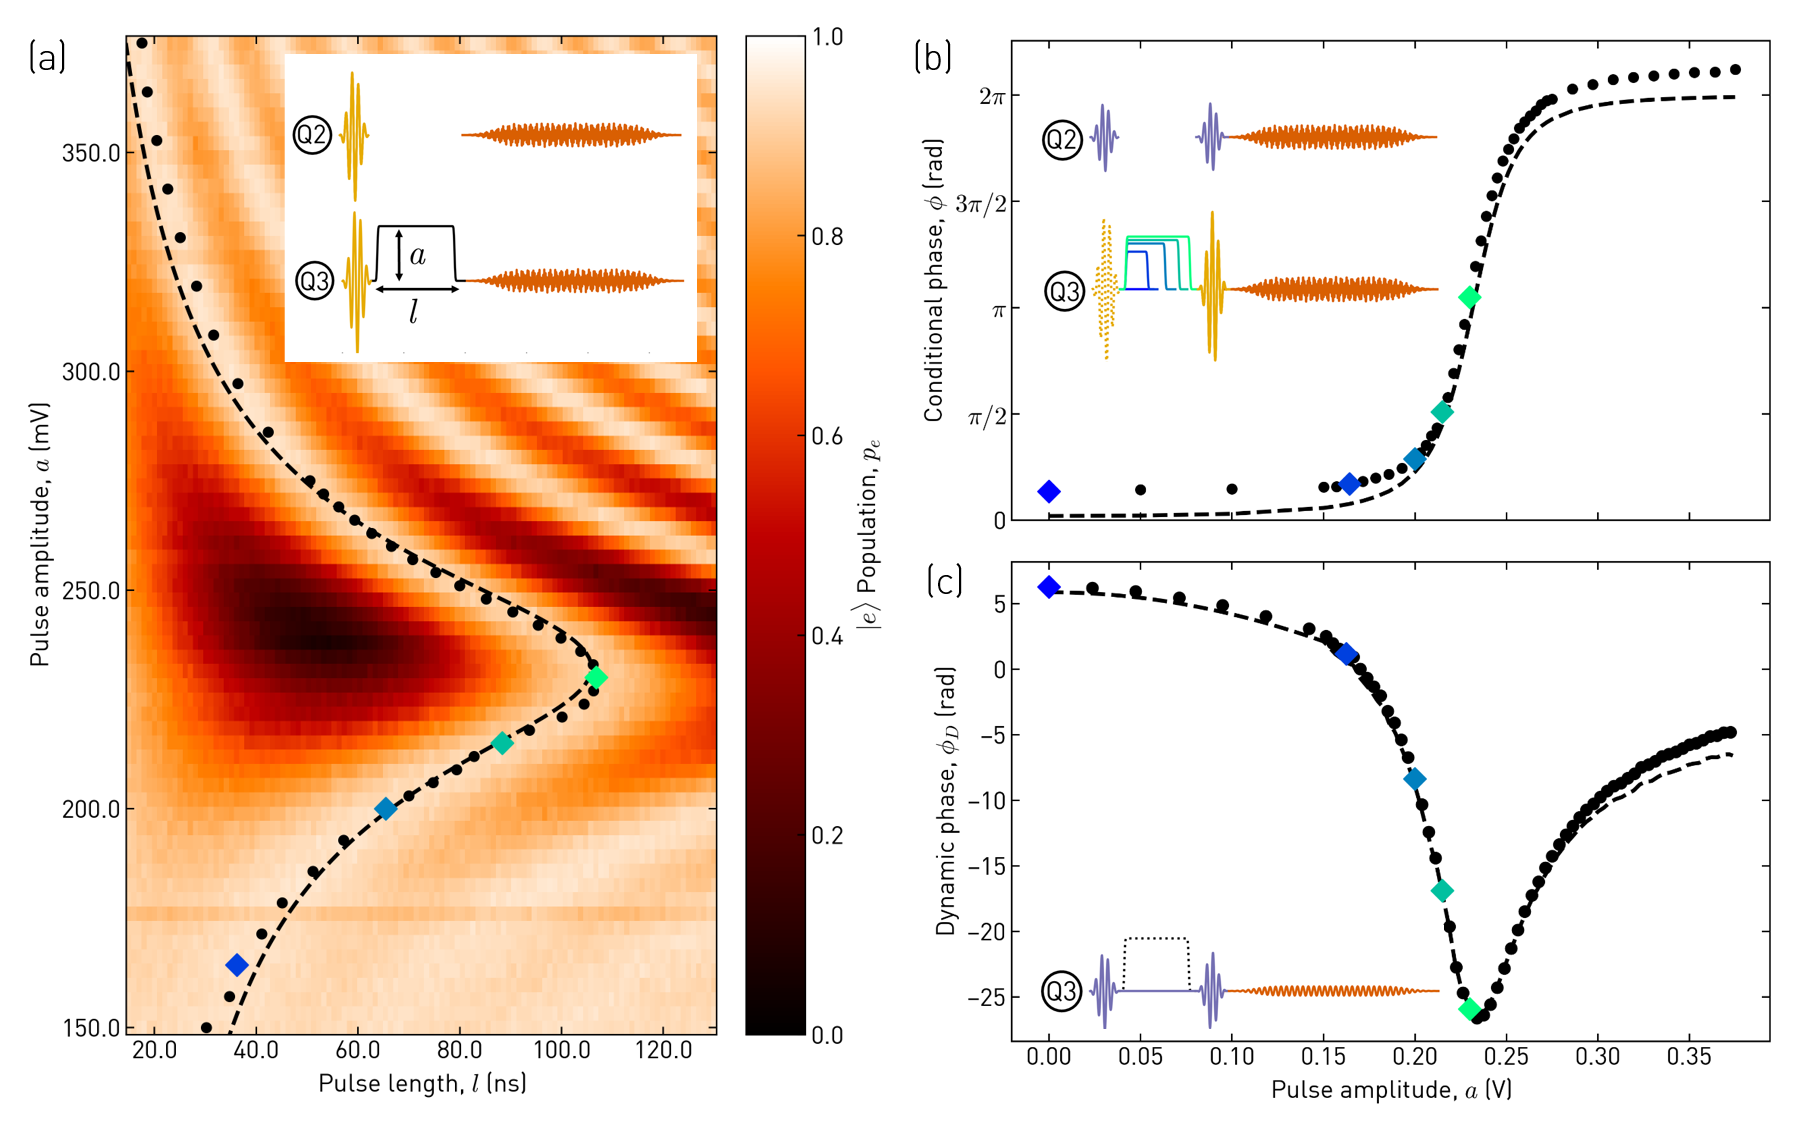
\includegraphics[width=\textwidth]{chapters/carb_gate/figs/ch4_calibration.png}
    \caption{Three calibration measurements of a \gls{carb} and their pulse schemes. Single qubit $R_x^\pi$, $R_x^{\pi/2}$ and readout pulse are shown in yellow, purple and orange respectively. A dashed pulse indicates the measurement is performed once without and once with the pulse. (a) Qubit 2 \e level population as function of the flux pulse amplitude and length. The inset details the pulse scheme: the \oo state is prepared, the flux pluse is  applied to qubit 3 (black), the two qubits are read out with a multiplexed readout pulse. The scattered points correspond to the amplitudes and lengths used to calibrate the conditional phase (see b). The dashed line corresponds to a fit to a theoretical model. (b) Conditional phase as function of flux pulse amplitude. The amplitude sampling is not uniform to account for the non linearity of the conditional phase. The dashed line indicates the phase prediction of the model. The phase is measured on qubit 2 with a Ramsey experiment, while qubit 3 is fluxed with and without preceding single qubit rotation. The difference between the two measurements yields the conditional phase. (c) Unwraped dynamic phase of qubit 3 as function of amplitude. Only one out of three data point is shown for clarity. The dynamic phase is measured by comparing the qubit phase with and without flux pulse. The dashed line corresponds to the predicted dynamic phase by theory.}
    \label{fig:ch4_calibration_carb}
\end{figure}


* Dynamic phase:
- brief recap dynamic phase is. Model. Approximation of square pulse.
- has to be calibrated if gate is to be used in algorithm. We add z gates to compensate for it. 
- calibration scheme: pi half + flux + pi half (i.e. ramsey experiment). (with and without flux?)
- Requires calibration for all possible lengths/amplitudes. Rrequires above niquist sampling rate.
See from model which sampling rate is required.

General discussion on calibration: time.

Link to next: investigate performance, leakage and stability required for use in algorithm.

\section{Characterization/ Benchmarking}
First step is to perform process tomography. Show one in fig + other angles in table or plot. 
Note: has to say that remove leakage. Justification: leakage has unpredictable effect on tomography since not in comp subspace. 
Hence 3L RO, RM F level and consider leakage separately. TODO: ref on influence of leakage in process tomo?
Non clifford --> cannot use RB ? 
Cross entropy Benchmarking: why good and why not?

 C- and D-phase errors: change to gate error. Fig: two in 1?
 Leakage over phi: Discuss tendencies and causes. FIR filters. Length of interaction.
 Process tomography
Time drift (combine this with prev?): Stable over time.